\documentclass{article}

% Language setting
% Replace `english' with e.g. `spanish' to change the document language
\usepackage[english]{babel}

% Set page size and margins
% Replace `letterpaper' with `a4paper' for UK/EU standard size
\usepackage[letterpaper,top=2cm,bottom=2cm,left=3cm,right=3cm,marginparwidth=1.75cm]{geometry}

% Useful packages
\usepackage{xcolor} % For color in the text
\definecolor{astana}{RGB}{220,220,220}
\definecolor{gray}{RGB}{128,128,128}
\definecolor{red}{RGB}{255,0,0}
\usepackage{makecell}
\usepackage{multirow}
\usepackage{amsmath} % For math
\usepackage{subcaption} % For subfigures
\usepackage{fancyhdr}
\usepackage{amsmath}
\usepackage{graphicx}
\usepackage[colorlinks=true, allcolors=blue]{hyperref}
\usepackage{titlesec}
\usepackage{enumitem}
\usepackage{amssymb}
\usepackage{amsthm}
\usepackage{tikz}
\usepackage{pgfplots}
\usepackage{float}
\usepackage{subcaption}
\usepackage{listings}
\usepackage{color}

\title{\vspace*{-3cm} % Adjusted to reduce the top margin
      \begin{center}
            \hspace*{0cm} % Adjusted to extend the black strip to the left
            \begin{tabular}{l@{}c@{}r}
                  \begin{tabular}{@{}c}
                        \textbf{Problem Chosen} \\
                        \textcolor{red}{\textbf{C}}
                  \end{tabular} &
                  \begin{tabular}{@{}c}
                      \textbf{2024} \\
                      \textbf{MCM/ICM} \\
                      \textbf{Summary Sheet}
                  \end{tabular} &
                  \begin{tabular}{@{}c}
                      \textcolor{black}{\textbf{Team control number}} \\
                      \textcolor{red}{\textbf{2417022}}
                  \end{tabular}
            \end{tabular} \\[0.3cm]
            \rule{\linewidth}{2pt} % Adjust the width and height here
            \vspace{-2.5cm} % Adjusted to reduce the bottom margin
      \end{center}
      \vspace{2cm}
      \textbf{\LARGE Uncover the secrets behind Alcaraz's success in Wimbledon}
}

\date{} % Removes the date
\author{} % Removes the author

\begin{document}
\maketitle
\begin{center}
      \Large\textbf{Abstract}
\end{center}
Abstract goes here.

% Define header and footer
\pagestyle{fancy}
\fancyhf{} % Clear default header and footer
% Header
\fancyhead[L]{\textit{Uncover the secrets behind Alcaraz's success in Wimbledon}} % Left-aligned header content

% Footer
\fancyfoot[C]{\thepage} % Centered page number
\fancyfoot[L]{\textcolor{gray}{2024 MCM/ICM C 2417022}} % Left-aligned footer content
\fancyfoot[R]{\textcolor{gray}{}} % Right-aligned footer content

\newpage
\tableofcontents % Table of contents
\newpage

\section{Introduction}
\subsection{Background}
Tennis originated in the 13th century in France. As early as the 16th to 17th centuries, French missionaries often played a game similar to tennis in the corridors of churches, using their hands to strike a small ball,
providing a diversion from the monotonous church life. Now, modern tennis has formally developed and quickly gained popularity in Europe and America, becoming a widely loved sport. [1] Tennis, as a charming and elegant sport, enjoys a high reputation and strong influence internationally. [2] With the continuous development of tennis, the fluctuations in the scores of opponents have become increasingly scrutinized during tennis matches. Recently, in the men's singles final at Wimbledon in 2023, 20-year-old Spanish rising star Carlos Alcaraz defeated 36-year-old Novak Djokovic, ending Djokovic's winning streak at Wimbledon since 2013. The twists and turns in the score and the changing dynamics of the match attracted significant attention. Therefore, effectively exploring the impact of the "momentum" on the score during the game is crucial.

\subsection{Problem restatement}
\begin{enumerate}
\item  Develop a mathematical model to quantify and visualize the progression of tennis matches, identifying key performance metrics for players during specific time intervals, with a particular focus on the service advantage.
\item Construct a statistical framework to assess the impact of momentum within a match, challenging the notion that players' swings in performance are random, and providing empirical evidence for or against this assertion.
\item Formulate a predictive model capable of indicating potential shifts in match dynamics, utilizing data from previous matches to identify indicators that signal when the flow of play may change in favor of one player over another.
\item Execute a comprehensive testing protocol for the aforementioned models across a series of matches, evaluating the predictive capabilities with respect to different match conditions, and identifying additional variables that may enhance future model iterations. Analyze the generalizability of the models to other match formats and sporting contexts, such as women's tennis, various tournaments, court surfaces, and racket sports akin to table tennis.
\end{enumerate}
\subsection{Our Work}
Firstly, the choice of model should be grounded in the context of the problem, taking into account the importance of momentum in tennis matches and its impact on player performance. Therefore, the model needs to capture the dynamic changes during a match and reflect the performance of players at different points in time. Factors such as scoring probability, fatigue levels, technical skills, and the mental state during the match are crucial indicators of momentum change, so the chosen model should integrate these factors to predict the scoring probability of players. Given that the dataset provides detailed match scores and other relevant statistics, machine learning algorithms like LGBM and XGBOOST are suitable choices because they can handle a large number of features and are applicable to classification problems. Moreover, considering the sequential nature of scoring in tennis matches, time series analysis or Hidden Markov Models could be used to capture the momentum changes throughout the match.
Taking all these factors into account, opting for gradient boosting algorithms (such as LGBM or XGBOOST) for modeling is a wise decision. These algorithms perform well in dealing with complex relationships and nonlinear patterns and can manage large datasets efficiently. Additionally, incorporating sequence models to capture temporal momentum changes should also be considered. The final model selection will be based on predictive accuracy (metrics such as accuracy, recall, precision, F1 score, AUC, and ROC curves) and the model's interpretability. Such a model will be able to assess the impact of "momentum" on the probability of scoring for players and provide insights into the presence of non-random fluctuations in matches.
\section{Problem Analysis}
In the first study, multiple key factors affecting the scoring abilities of tennis players were comprehensively considered. This included not only whether they were serving but also factors like their level of fatigue, technical skills, and psychological state during the match. A comprehensive evaluation system was designed to deeply analyze these variables, such as individual technical levels, degrees of fatigue, and real-time mental states during matches. By employing statistical Logistic regression, the proposed system of indicators was tested for its correlation with players' scoring, and its effectiveness was validated on a dataset of tennis matches. Machine learning techniques, including LGBM, XGBOOST, support vector machines, perceptron networks, and logistic regression, were applied along with five-fold cross-validation and multi-dimensional performance metrics. The gradient boosting algorithm LGAM was ultimately chosen to dynamically assess players' real-time performance, or what is referred to as match "momentum."

The second study focused on exploring whether the "momentum" effect during matches has statistical significance, that is, whether the fluctuations in players' scoring during matches are non-random. The optimized machine learning model developed in the first study was applied to a test dataset, with predicted scoring probabilities compared to actual scoring records of athletes, and validated through Pearson correlation analysis. Subsequently, a univariate linear regression model was established, using predicted "momentum" as the independent variable and players' scoring as the dependent variable, to quantify the impact of "momentum" on scoring.

The third study addressed the challenges of model construction, as the model from the first study primarily focused on predicting the scoring probability of each serve and shot, rather than volatility prediction. To bridge this gap, the predictive focus was adjusted from individual shots to the outcome of entire games, analyzing fluctuations in players' performances across individual sets and the entire match. By aggregating features, a predictive model was built using statistical Logistic regression, with the support vector machine chosen as the final model. Model performance was evaluated using LGBM, XGBOOST, recall, precision, F1 score, AUC, and ROC curves. The information gain method was employed to determine the importance of various variables in the indicator system, leading to recommendations for athletes' future performance in matches.

In the final study, by selecting four matches as a validation set and using other match data as a training set, the visualization method of the ROC-AUC curve showcased the model's performance differences across various matches. Considering the uncertainty of the "volatility" indicator, machine learning evaluation standards were used for performance evaluation. In tests across these four matches, the constructed model demonstrated significant performance differences. Given this, expandable research directions were proposed, emphasizing the importance of individual athlete abilities and proving the applicability and strong generalizability of the proposed indicator system in other competitions


\section{Model Assumption}
\begin{enumerate}
\item The server has a greater advantage over the receiver.This assumption posits that the player initiating the serve in a game is more likely to gain an upper hand.
\item Players are affected by the "momentum" of the match.It's assumed that the success or failure of players during a match influences their future performance, suggesting that momentum plays a critical role in the outcome of the game.
\item A player's technical skill has a significant and direct impact on their scoring performance.This assumption highlights the importance of individual skills and how they translate into points on the board.
\item Fatigue affects players during the match, impacting their performance in the later stages.This suggests that as the match progresses, players' energy levels and their ability to maintain peak performance diminish.
\item The psychological state of players, including their ability to handle mistakes and respond to critical moments, significantly influences the match.This assumption underscores the importance of mental toughness and psychological preparedness in determining a player's success in competition.
\end{enumerate}
\section{Symbol Description}
\begin{table}[H]
\centering
\begin{tabular}{|>{\centering\arraybackslash}m{2.5cm}|p{0.6\textwidth}|}
\hline
\textbf{Symbol} & \textbf{Description} \\ \hline
$S1$ & The number of game winning in the current set \\ \hline
$S2$ & The leading scores in the current game \\ \hline
$S3$ & Whether it is the server \\ \hline
$S4$ & Whether score in the last point \\ \hline
$S5$ & The score lead progress of this match\\ \hline
$S6$ & Whether the serve is scored (no contact) \\ \hline
$S7$ & Whether to score on a return kick (no touch). \\ \hline
$S8$ & No touch score on the backhand \\ \hline
$S9$ & Is there a double fault in this game? \\ \hline
$S10$ & Whether there were unforced errors in this game. \\ \hline
$S11$ & The ratio of the number of net to the number of times score by net \\ \hline
$S12$ & The ratio of the chance of scoring when the opponent serves to the number of points actually scored. \\ \hline
$S13$ & Total mileage in this match \\ \hline
$S14$ & The total mileage in the last three points \\ \hline
$S15$ & Mileage chart from last point \\ \hline
$S16$ & Serve real-time pace \\ \hline
\end{tabular}
\caption{Symbol Description}
\end{table}
\section{Model Construction and Analysis}
\subsection{Task1's Model}
\subsubsection{Data Preprocessing}
In the initial phase of data preprocessing, the dataset is imported from a .csv file, and the Pandas library is employed to structure the data into a DataFrame. Subsequent to this, the dropna function is applied to eliminate records with missing values. Following the initial data preparation, the script undertakes a comprehensive feature engineering process, introducing novel features pertinent to the distinct characteristics of tennis matches.

In the subsequent phase, the dataset is readied for modeling through a meticulous iteration over each data point. This involves the extraction of features and the assignment of labels contingent upon the outcome of each point, specifically focusing on point victories. To enhance the robustness and suitability of the data for subsequent machine learning applications, the features undergo scaling. The MinMaxScaler from the scikit-learn library is employed for this purpose, ensuring that all variables are standardized within the [0, 1] range. This standardization is imperative to mitigate the undue influence of certain features during the modeling process, arising from variations in scale.

The finalization of the preprocessing sequence involves the preservation of the processed and standardized dataset in an Excel file. These methodical steps collectively address challenges associated with missing values, outliers, and standardization, culminating in the generation of a refined dataset poised for efficacious utilization in machine learning endeavors.
\subsubsection{Model Analysis}
The analysis of player performance in tennis is a multifaceted task that requires a comprehensive approach, blending traditional statistical methods with advanced machine learning techniques. In this section, we delve into the intricacies of our model, examining the preprocessing steps, model training, evaluation metrics, and the overall performance against various benchmarks.

Initially, we employed logistic regression to assess the statistical significance of the relationship between our established indicator system and the corresponding labels. Leveraging a tennis match dataset, we computed these indicators and labels indicating player scoring. This step not only aids in comprehending how various factors impact a player's score but also lays a crucial groundwork for feature selection in the modeling phase.

Subsequent to this, we utilized a range of machine learning algorithms, including LGBM, XGBoost, Support Vector Machines, Perceptron Networks, and Logistic Regression. We compared their effectiveness using metrics like accuracy, recall, precision, F1-score, AUC, and ROC curves. This step not only robustly supports our final choice of the LGAM algorithm for modeling but also ensures the model's capacity for generalization.

In the concluding phase, we opted for the LGAM algorithm for modeling. This algorithm not only dynamically evaluates a player's performance but also captures shifts in "momentum" during a match. This dynamic assessment model facilitates more accurate predictions of a player's performance, enhancing the precision of predicting match outcomes. Through this research, we have taken a noteworthy stride in comprehending and appraising player tactics and scoring, establishing a strong basis for more in-depth analysis and prediction.

Concerning the creation of the indicator system, we analyzed potential factors influencing a tennis player's scoring. The system was formulated based on elements like player fatigue, real-time and historical scoring situations, and the player's psychological state. This thorough analysis contributes to a nuanced understanding of player performance, paving the way for further exploration and prediction.

\subsubsection{Index creation}
we analyze the factors that might correlate with the player's score. According to the player's fatigue and mental state etc., make an index system as follows.

\begin{table}[H]
      \centering
      \begin{tabular}{|>{\centering\arraybackslash}m{2.5cm}|p{0.6\textwidth}|}
      \hline
      \textbf{Categery} & \textbf{Index} \\ \hline
      Fatigue &  Total mileage in this match\\ \hline
      Fatigue &  The total mileage in the last three points \\ \hline
      Fatigue &  Whether score in the last point \\ \hline
      State & Whether there is a double fault \\ \hline
      State & Whether there were unforced errors in this game.\\ \hline
      State & Serve real-time pace  \\ \hline
      State & Whether it is an interactive item for the server's serving pace\\ \hline
      State &  The ratio of the number of net to the number of times score by net\\ \hline
      State & The ratio of the chance of scoring when the opponent serves to the number of points actually scored.\\ \hline
      Ability& Whether the serve is scored (no contact) \\ \hline
      Ability& Whether to score on a return kick (no touch). \\ \hline
      Ability& No touch score on the backhand \\ \hline
      Ability& The score lead progress of this match\\ \hline
      Ability& The leading scores in the current game \\ \hline
      Ability& The number of game winning in the current set \\ \hline
      Ability& Whether score in the last point \\ \hline
      Situations& Whether it is the server \\ \hline
      \end{tabular}
      \caption{Symbol Description}
\end{table}
\subsubsection{Statistical Logistic Regression Analysis Based on Indicator System}
This study employs a comprehensive indicator system to assess the impact of various factors on the real-time scoring of players in sports matches.
The indicator system allows for the calculation of scores for each point in every set of every match played by a participant, with corresponding assessments 
of the player's current performance indicators. To validate the significance of the indicators within this system concerning point scoring, a statistical regression analysis is conducted. 
Given the binary nature of point scoring outcomes, a binary logistic regression model is selected, and the analysis is executed using SPSS software.
\begin{figure}[H]
      \centering
      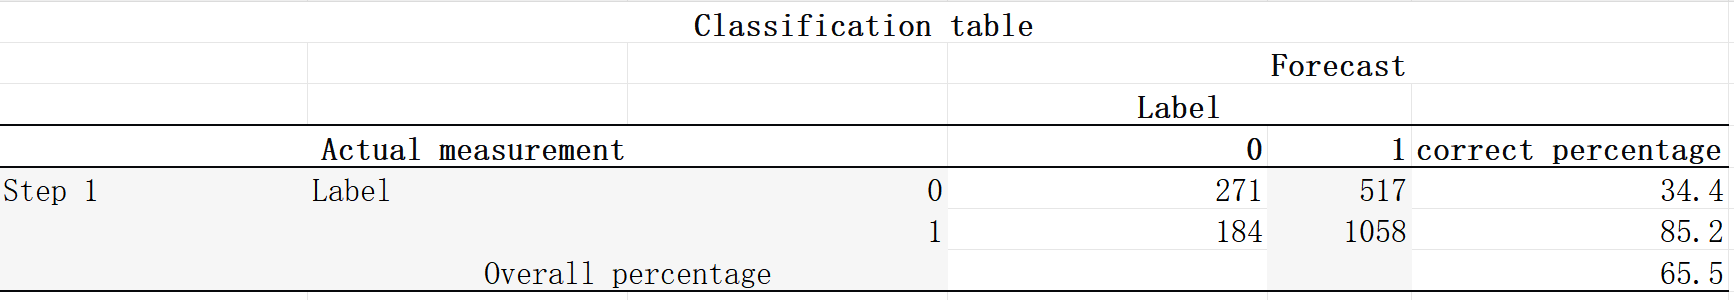
\includegraphics[width=0.7\textwidth]{logistic_classfication_1.png}
      \caption{logistic regression performance}
\end{figure}
The logistic regression analysis in SPSS yielded an overall accuracy of 65.5\%. The model exhibited a classification accuracy of 34.4\%
for instances where players genuinely did not score, while achieving a significantly higher accuracy of 85.2\% for instances where players did score. 
This suggests a preference of the model to classify samples into situations where players actually scored (label 1).

However, it is crucial to note that this logistic regression analysis provides a prospective examination. Its purpose is to investigate 
whether the constructed indicators significantly influence the actual scoring situation of players. The results of the logistic regression analysis are presented in the following table.

\begin{figure}[H]
      \centering
      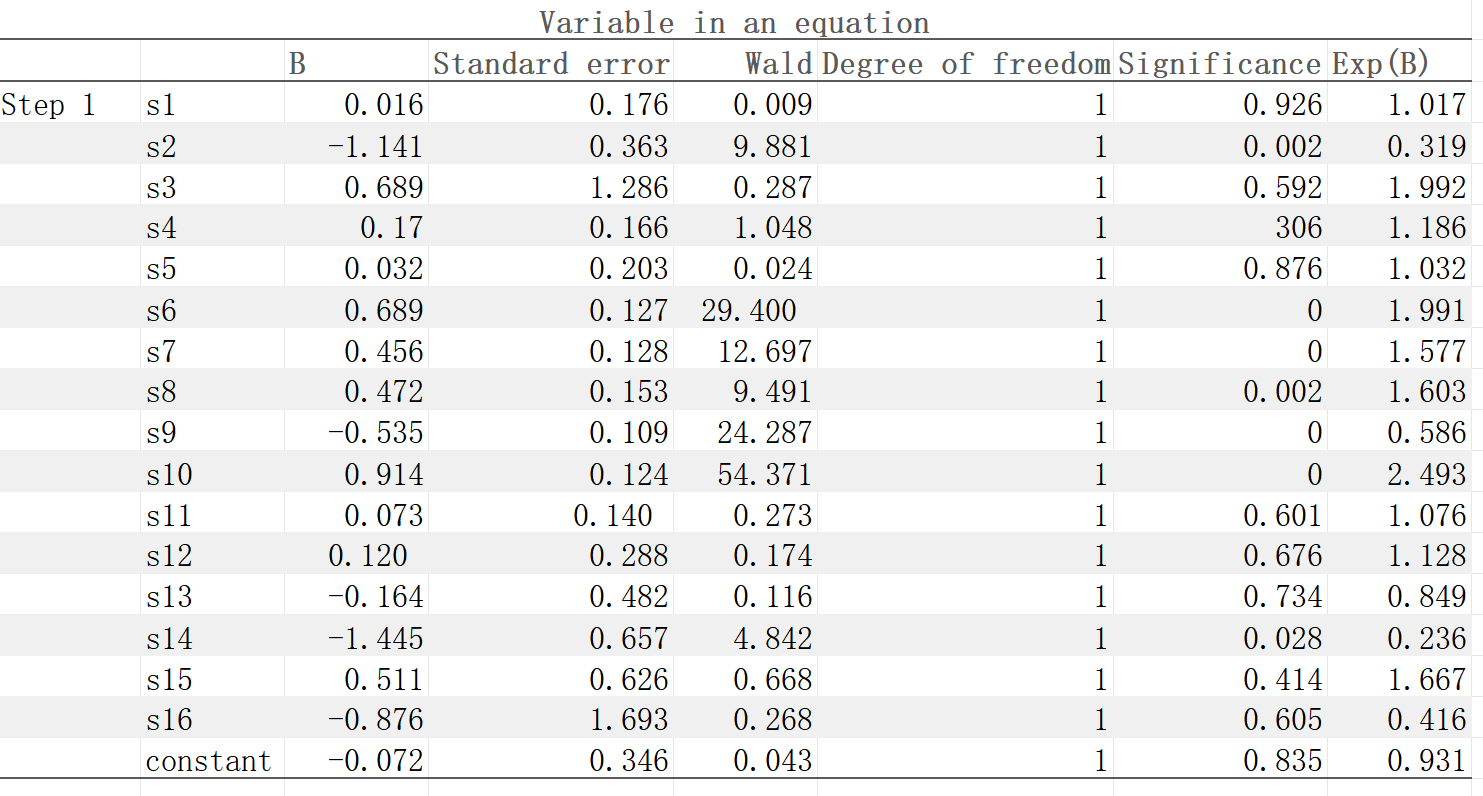
\includegraphics[width=0.7\textwidth]{variable_eq1.png}
      \caption{Logistic regression results}
\end{figure}
As the figure table shows, the p-values for the majority of the independent variables are less than 0.05, indicating a significant influence of these variables on the dependent variable. Consequently, in this indicator system, 
variables such as s2, s6, s7, s8, s10, and s14 have been identified as significantly affecting a player's real-time scoring situation. 
This suggests that both a player's individual abilities and factors like fatigue or psychological state can exert a significant impact on their real-time scoring performance.

\subsubsection{Evaluation of Machine Learning Models Based on an Indicator System}
The model construction phase involves the selection of high-performing ensemble tree models, specifically LightGBM (LGBM) and XGBoost, alongside classical machine learning algorithms, 
namely Support Vector Machine (SVM), Perceptron Neural Network, and Logistic Regression, serving as comparative benchmarks. The models are validated using k-fold cross-validation, 
and performance metrics such as accuracy, precision, recall, F1 score, and AUC-ROC curve are derived from confusion matrices.

The confusion matrix-based results are presented in the table below, while the training and testing outcomes based on AUC-ROC curves are illustrated in the figures.
\begin{figure}[H]
      \centering
      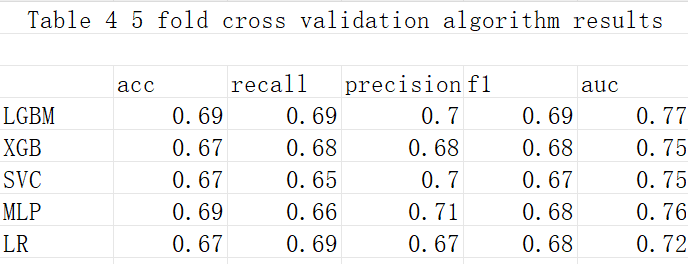
\includegraphics[width=0.7\textwidth]{cross_valadation.png}
      \caption{Cross Valadation}
\end{figure}

Among the models, LGBM exhibits superior performance with accuracy, precision, recall, F1 score, and AUC values of 0.69, 0.69, 0.77, 0.69, and AUC\_L respectively. Neural Network follows closely, demonstrating minimal discrepancies in metrics (0.69, 0.66, 0.71, 0.68, AUC\_NN), indicating a lack of pronounced bias in positive or negative sample discrimination. Consequently, the effectiveness of LGBM is affirmed.
\begin{figure}[H]
      \centering
      \begin{subfigure}{0.48\textwidth} % Adjust the width as needed
          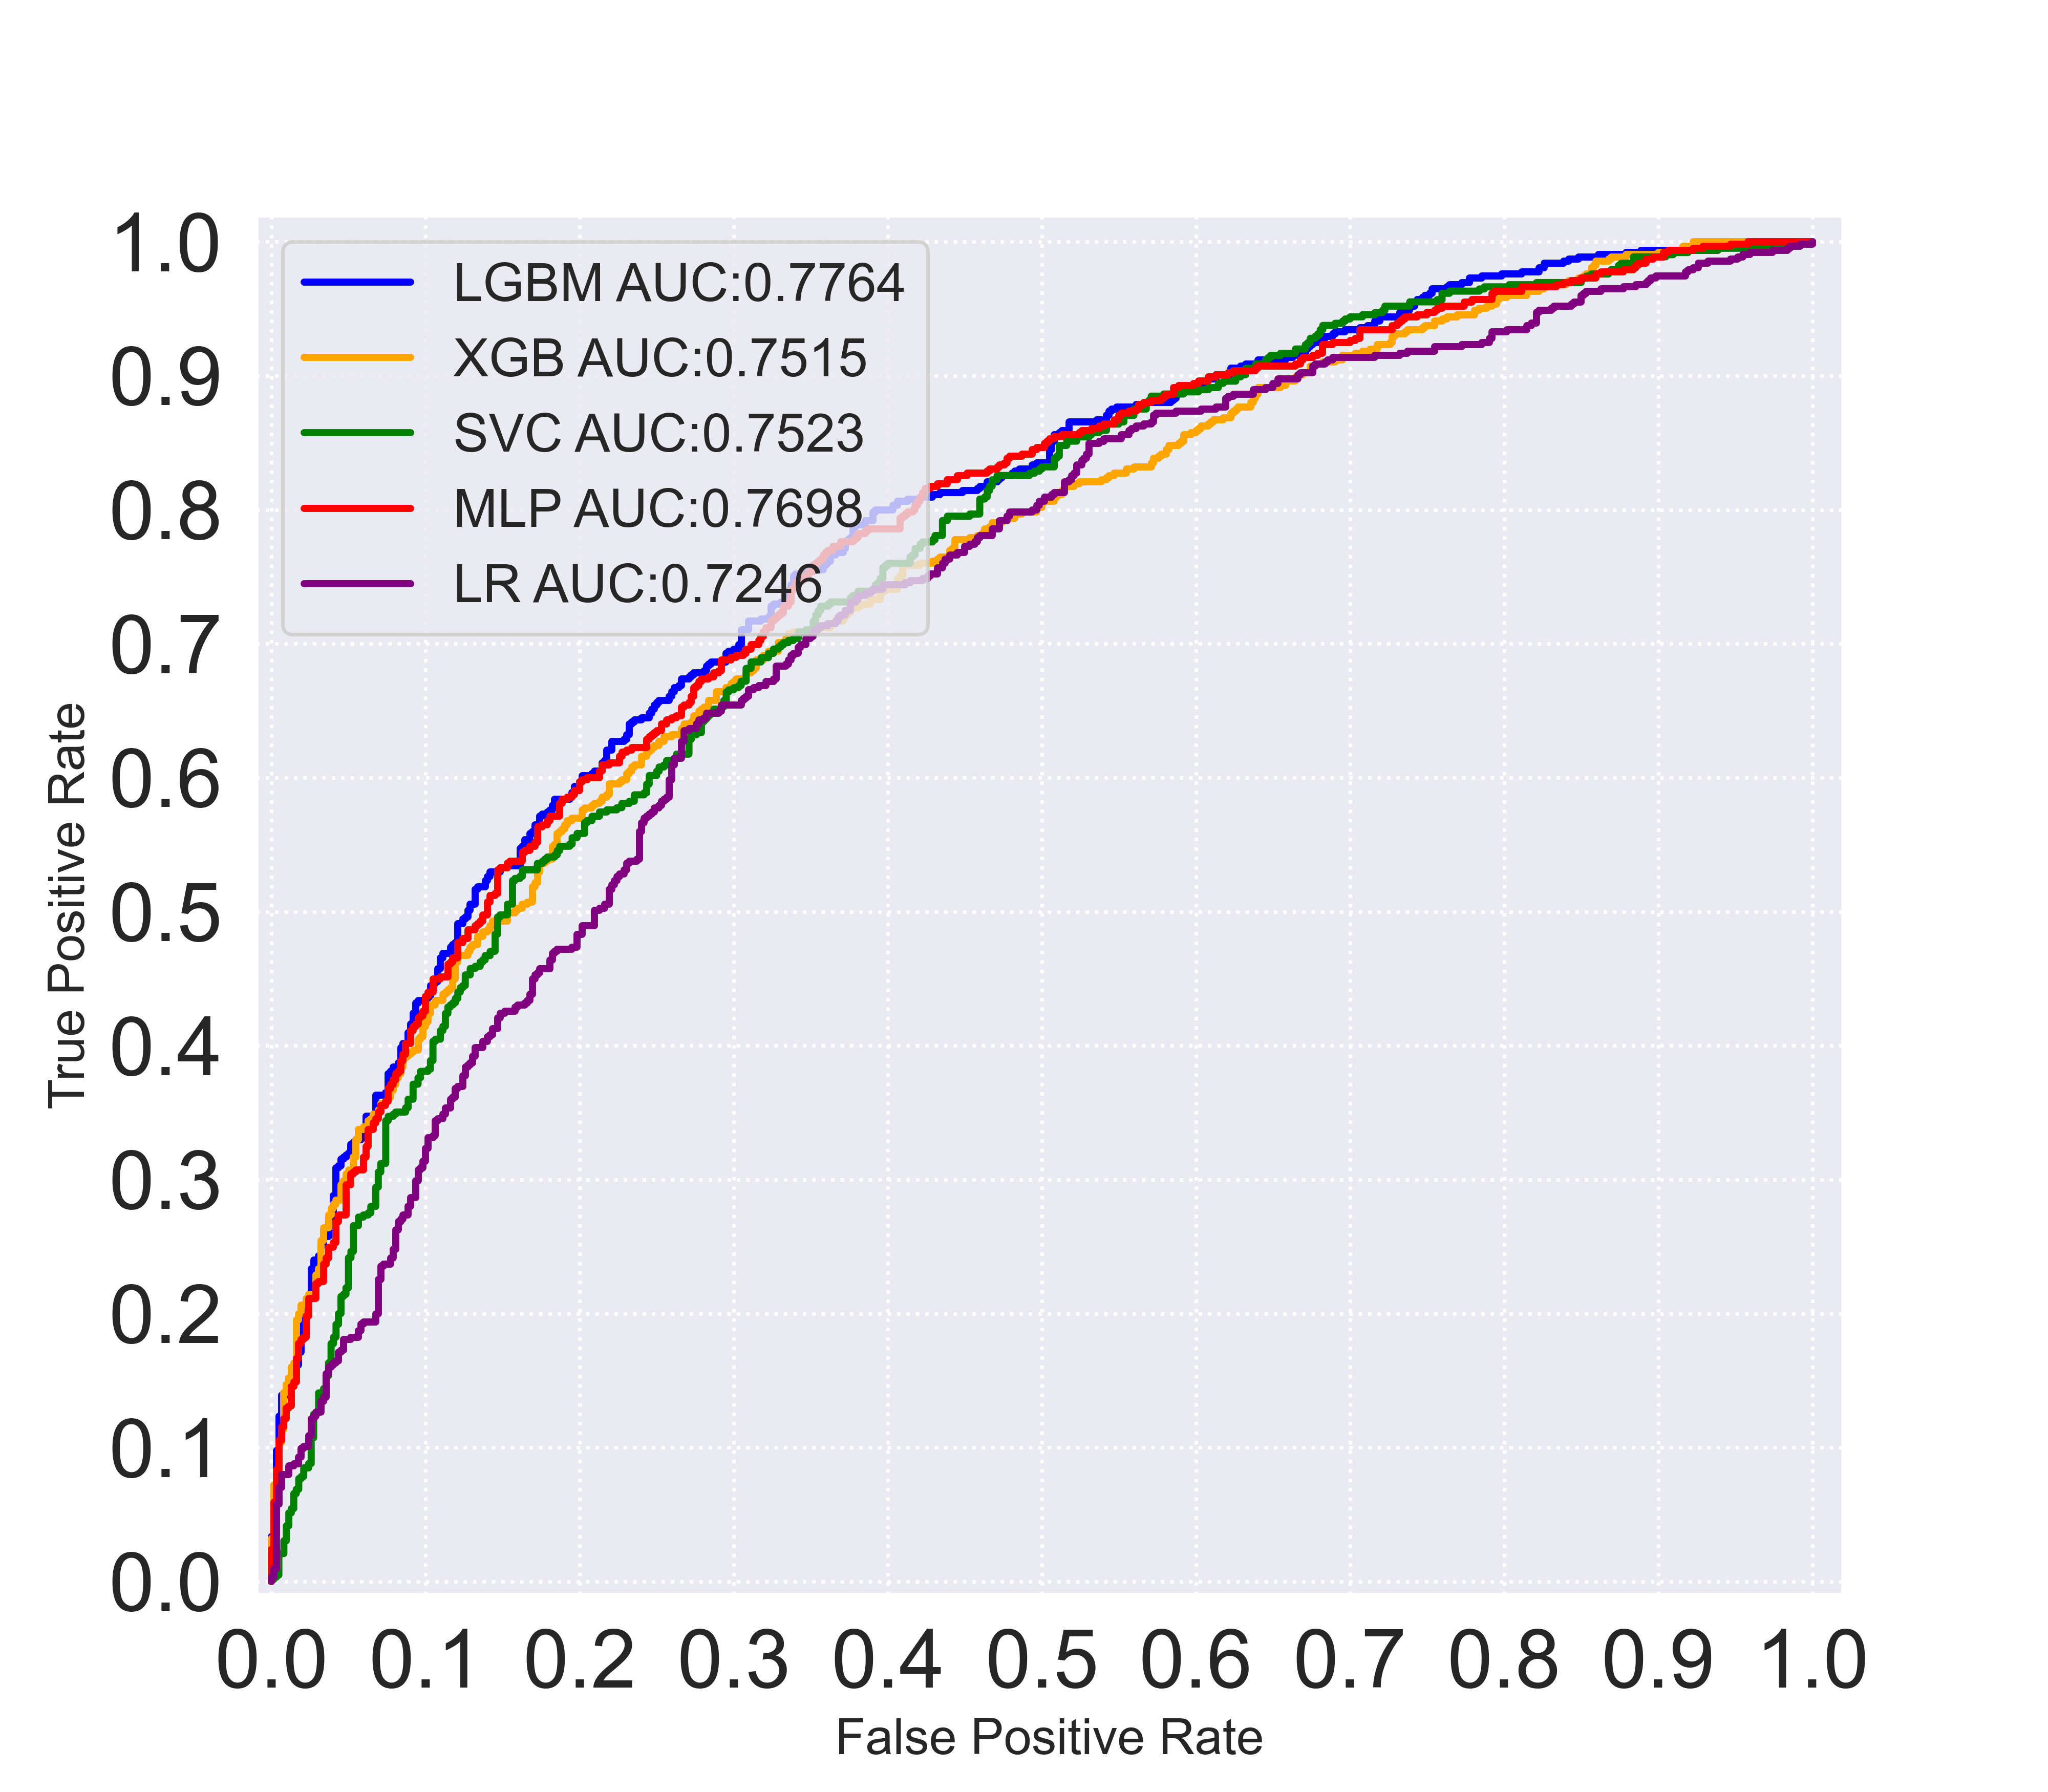
\includegraphics[width=\linewidth]{roc_auc(test(before_sampling)).png} % Replace 'figure1' with the filename of your first figure
          \caption{Test}
          \label{fig:roc_test}
      \end{subfigure}
      \hfill % Add horizontal space between the subfigures
      \begin{subfigure}{0.48\textwidth} % Adjust the width as needed
          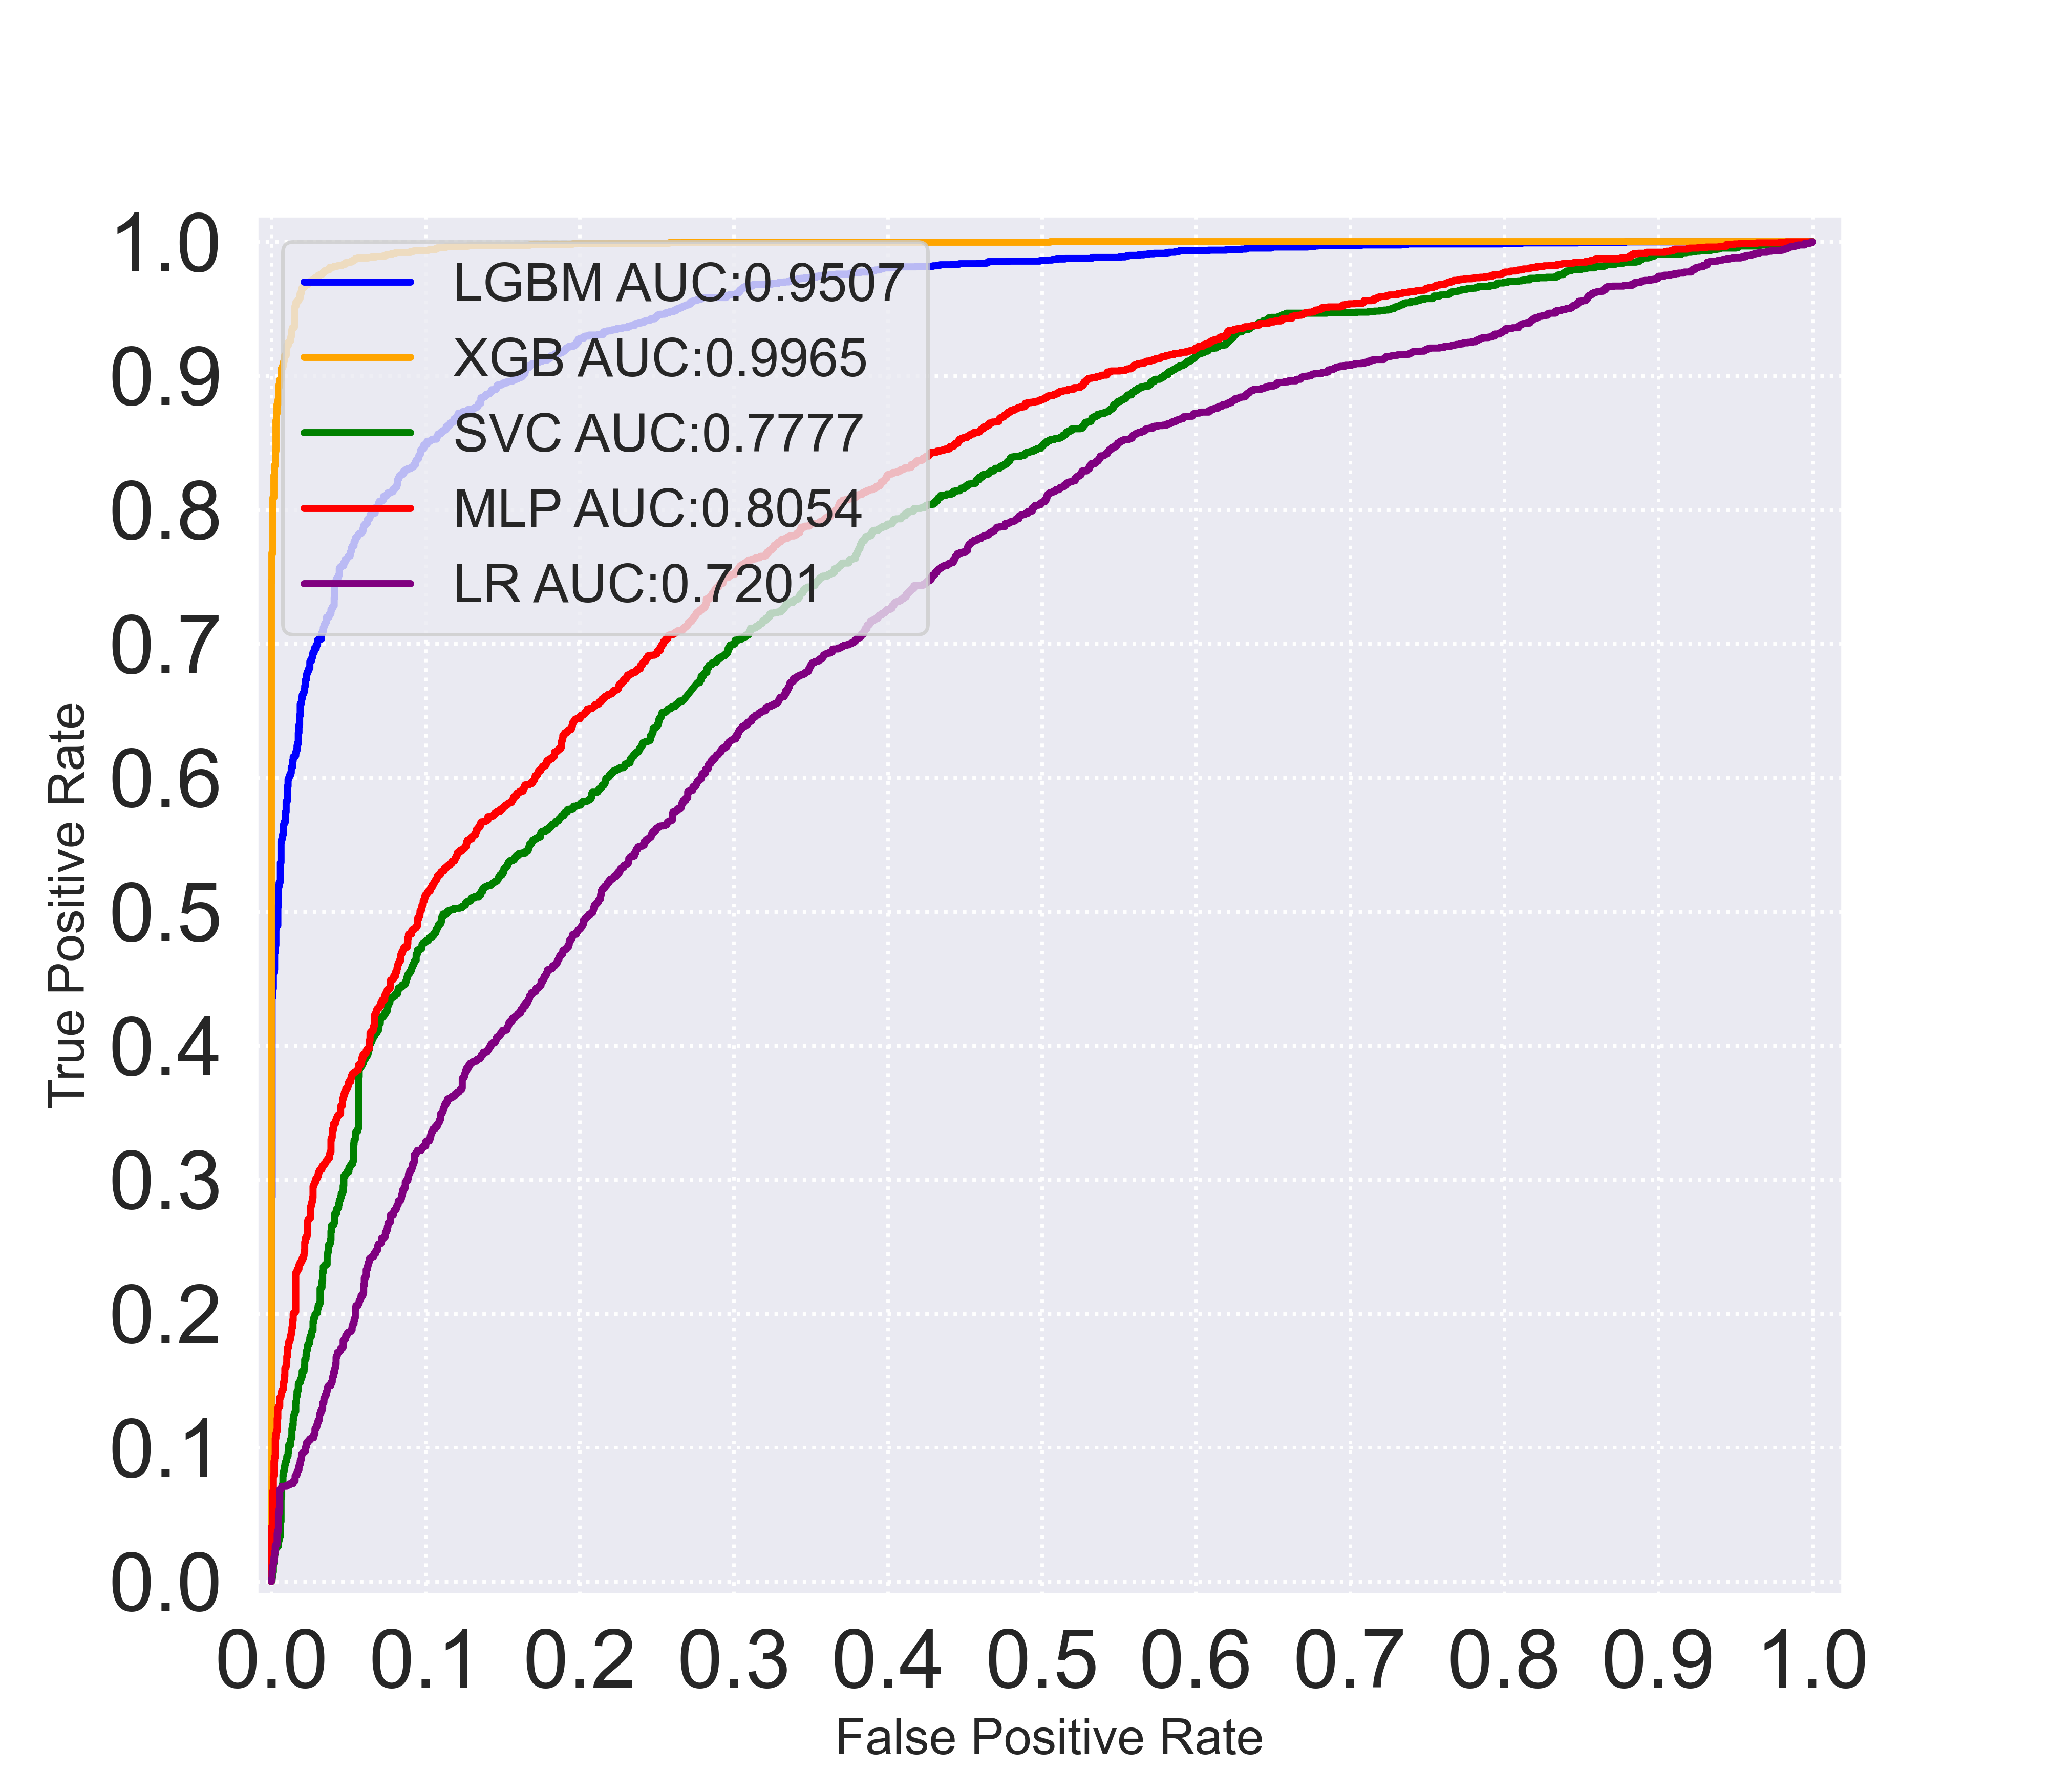
\includegraphics[width=\linewidth]{roc_auc(train(before_sampling)).png} % Replace 'figure2' with the filename of your second figure
          \caption{Train}
          \label{fig:roc_train}
      \end{subfigure}
      \caption{Task 1 Overall performance of the model}
      \label{fig:overall}
\end{figure}

The ROC curves illustrate variations in precision and recall metrics at different threshold settings. Through ROC analysis, it further validates LGBM as the most effective algorithm.

Building upon these findings, a new training model is established utilizing the top-performing LGBM model. Real-time performance visualization is conducted on the classic match between 20-year-old rising Spanish star Carlos Alcaraz and 36-year-old Novak Djokovic in the 2023 Wimbledon Men's Singles Final. The result is shown as follows.
\begin{figure}[H]
      \centering
      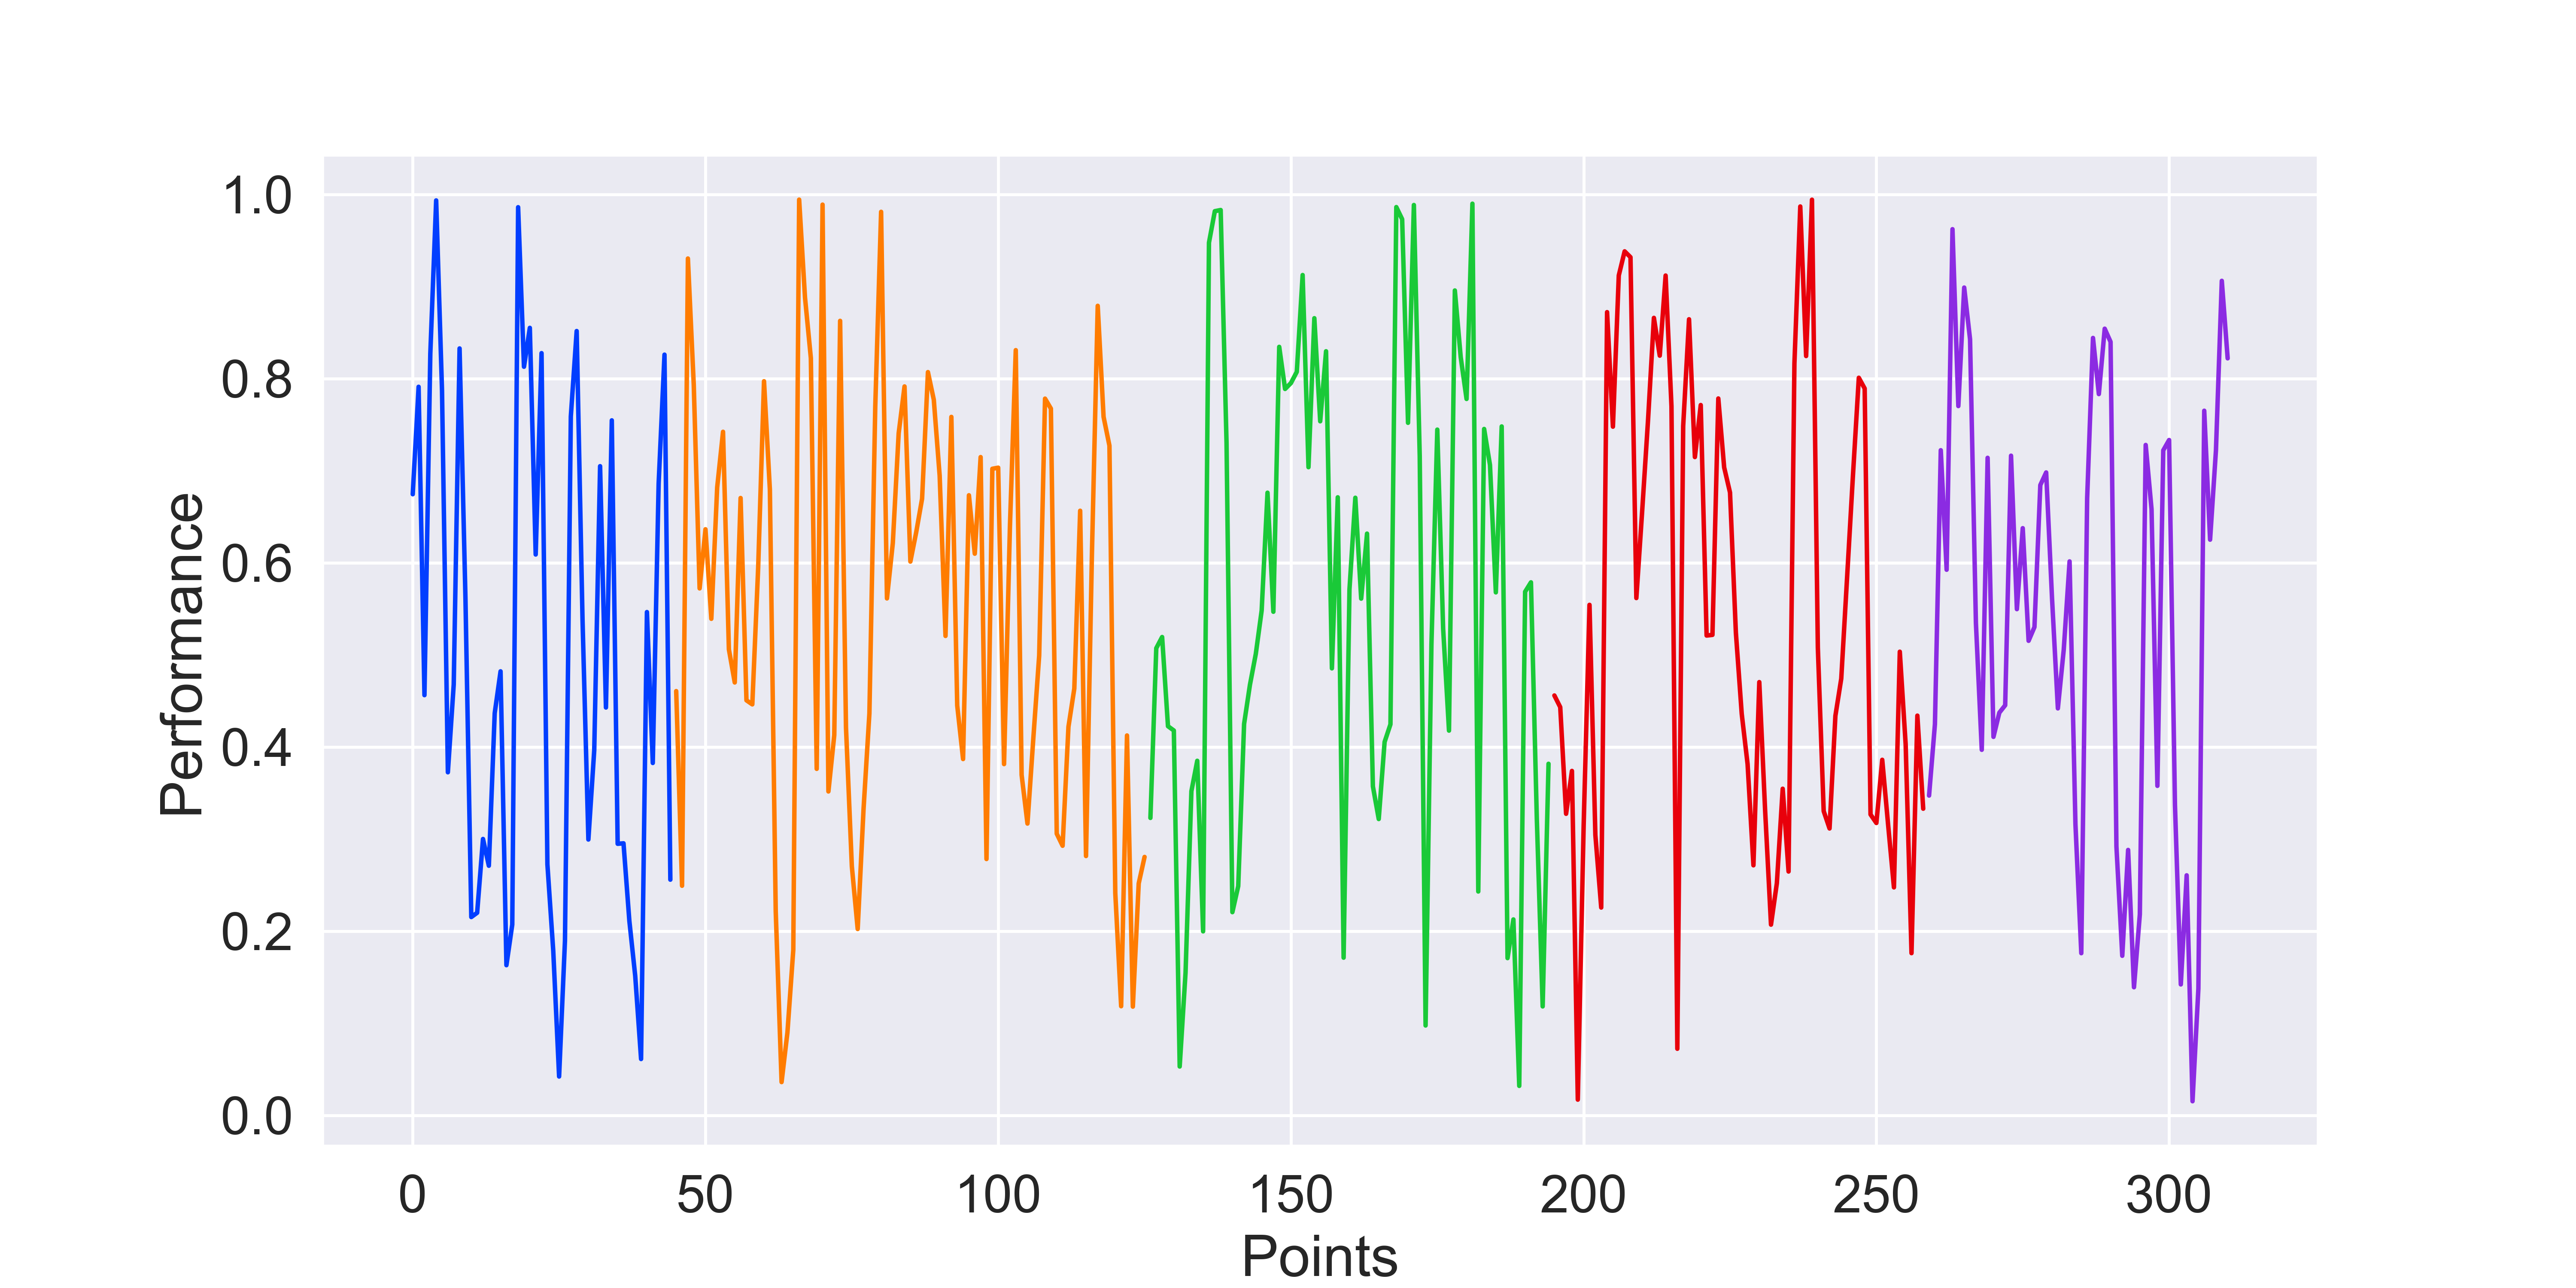
\includegraphics[width=0.7\textwidth]{classic_duel_trend.png}
      \caption{Classic duel}
\end{figure}

In fact, the predictive accuracy for scoring points has no upper limit, which aligns with our intuition. The complexity of factors influencing whether a player can score is highly intricate. 
Without considering these complex elements, the noise in a player's performance becomes significantly pronounced. As a result, the model can accurately discern the real scoring situations of only approximately 70\% 
of the players. We observe that in this classic match, the server and scorer precisely align with the actual scoring situations of the players. When Carlos Alcaraz secures victory, the momentum is high, and it is relatively low when facing defeat. 
This indicates that the model remains effective, as it reflects the consistency between the classic battle outcomes and the real-time scoring situations of the players.
\subsection{Task2's Model}
\subsubsection{Task2's Model Analysis}
In the second phase of our research, we are dedicated to gaining a deeper understanding of the practical role of "momentum" in sports competitions. The aim is to unveil whether the fluctuations and successes exhibited by players during a match demonstrate a non-random trend. 
To achieve this objective, I initially applied the optimal machine learning model established in question one to the test set, generating probability outputs for player scoring. Through Pearson correlation tests between these outputs and the actual player scoring situations, 
we attempt to identify the degree of association between the output probabilities and the real scoring outcomes.

Furthermore, we employ a univariate linear regression model, where the predicted "momentum" serves as the independent variable and the player's actual scoring as the dependent variable. Through this modeling process, we not only track the impact of momentum on real-time scoring 
but also endeavor to uncover the interpretable components behind the "momentum." This in-depth analytical process aims to reveal the exact mechanisms through which "momentum" influences player scoring, providing a more comprehensive understanding of the dynamic characteristics of player performance.

Within this research framework, we anticipate concluding that "momentum" is not merely a simple random phenomenon but indeed exerts a noticeable and meaningful impact on player scoring. Through these efforts, we aim to offer a more detailed and profound insight into the practical significance 
of momentum in sports competitions, providing specific recommendations and guidance for player performance during matches.
\subsubsection{Pearson Correlation Test}
\textbf{Principles of Pearson Correlation Test}\\

The Pearson correlation coefficient is a statistical measure used to assess the linear relationship between two variables, with values ranging from -1 to 1. Specifically:

\begin{itemize}
  \item A value of 1 indicates a perfect positive correlation: when one variable increases, the other variable increases correspondingly.
  \item A value of -1 indicates a perfect negative correlation: when one variable increases, the other variable decreases.
  \item A value of 0 suggests no linear relationship.
\end{itemize}

The calculation formula for the Pearson correlation coefficient (often denoted by the symbol \(r\)) is as follows:

\[ r = \frac{\sum{(x_i - \bar{x})(y_i - \bar{y})}}{\sqrt{\sum{(x_i - \bar{x})^2} \cdot \sum{(y_i - \bar{y})^2}}} \]
\\
Here, \( x_i \) and \( y_i \) are the corresponding data points, \( \bar{x} \) and \( \bar{y} \) are the respective means of the variables. The numerator represents the sum of the product of the deviations of each data point from their respective means, while the denominator signifies the square root of the product of the sums of squared deviations for both variables.

A computed \( r \) value closer to 1 or -1 indicates a stronger linear relationship between the two variables. Conversely, an \( r \) value close to 0 suggests a lack of linear relationship between the variables.
\\
\textbf{Pearson Correlation Test Results}\\

As the goal is to demonstrate whether the momentum output by the model can influence the players' actual performance, it is necessary to establish the significance of their correlation.
\begin{table}[H]
      \centering
      \begin{tabular}{|c|c|}
      \hline
      \textbf{Correlation coefficient} & \textbf{P Value} \\ \hline
      0.482 &  0.000\\ \hline
      \end{tabular}
      \caption{Pearson result}
\end{table}
It is observed that the p-value is less than 0.05, indicating a significant correlation between momentum and player performance. Furthermore, this relationship is characterized as a positive correlation, signifying that a larger momentum corresponds to better player performance and an increased likelihood of scoring.

\subsubsection{Univariate Linear Regression Model}  
Similarly, we use linear regression to analyze whether momentum can significantly affect player scores. The result is as shown below:
\begin{figure}[H]
      \centering
      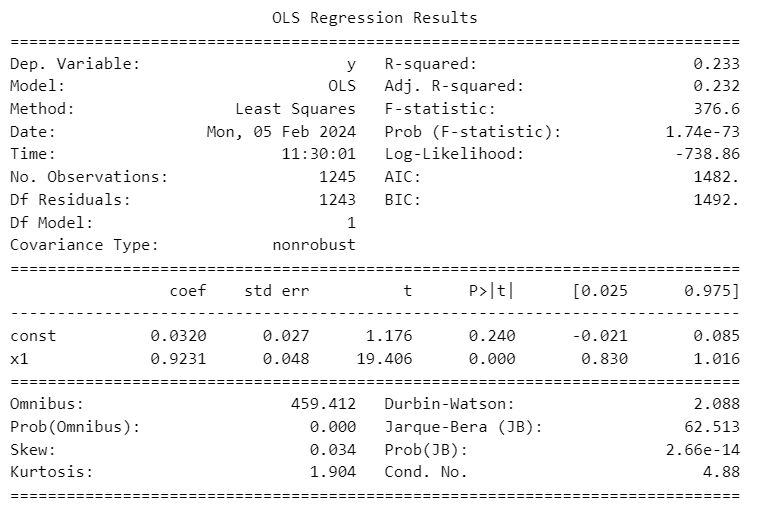
\includegraphics[width=0.7\textwidth]{Univariate_linear_regression.png}
      \caption{Univariate regression}
\end{figure}
It can be seen that the p-value of momentum is also less than 0.05, and its weight is 0.9231. The impact of momentum x1 on the results is significant, and it can explain 0.233 of the results.

\subsection{Task3's Model}
In the study of question three, we deeply analyzed the limitations of the established model. This model mainly focuses on predicting the score of each player's serve and stroke, and is therefore limited to having high randomness. ,To overcome one of the limitations, we adopted a ,more nuanced approach designed to more accurately reflect ,player performance fluctuations throughout the game.

First, we upgraded the model in Question 1 to aggregate features and calculate the player's single game win. This new prediction goal provides us with more specific and accurate data, allowing us to better understand Player performance in the game. Subsequently, we again used statistical LOGISTI to build a model to determine the significant impact of the proposed indicator system on predicting game results.

Comparing the results of Question 1, we found that the indicator system proposed in the text has a more significant impact on the independent variables in game prediction. In the comparative analysis of multiple machine learning algorithms, especially LGBM, XGBOOST, support vector machine, perceptron network, and logistic regression, the support vector machine performed well and became the best model we selected. In order to further strengthen the model For interpretability, we used the information gain method to calculate the importance score of the indicator system, which helps us understand the specific contribution of each indicator to the players.

In the end, we not only provided an excellent support vector machine model for modeling player performance fluctuations, but also gained a deeper understanding of the importance of the indicator system through the analysis of information gain. At the end of the study,
we provide performance recommendations for players when entering new games, aiming to help players achieve better performance in the game. These recommendations are not only based on our model results, but also incorporate the overall status of the players and specific 
situations. Deep insights provide players with more comprehensive support.

\subsection{Logistic test with game as granularity}
Similarly, we use statistical logistic regression for testing. The results are shown in the table
\begin{figure}[H]
      \centering
      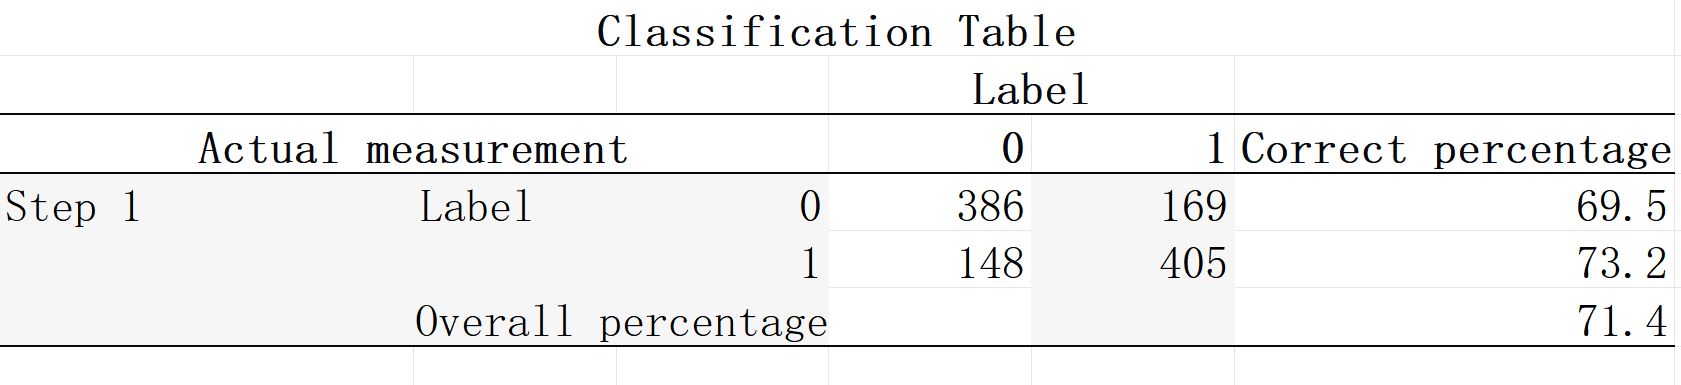
\includegraphics[width=0.7\textwidth]{logisitc_classification2.png}
      \caption{Logistic regression performance}
\end{figure}
It can be seen that compared to point-based logistic regression, the accuracy of game-based logistic regression has a clear value-added, 
from 65.5 to 71.4. At this time, the results of the model can better reflect the real fluctuation state of the players. Then, the results of the logistic 
regression test are as shown in the figure
\begin{figure}[H]
      \centering
      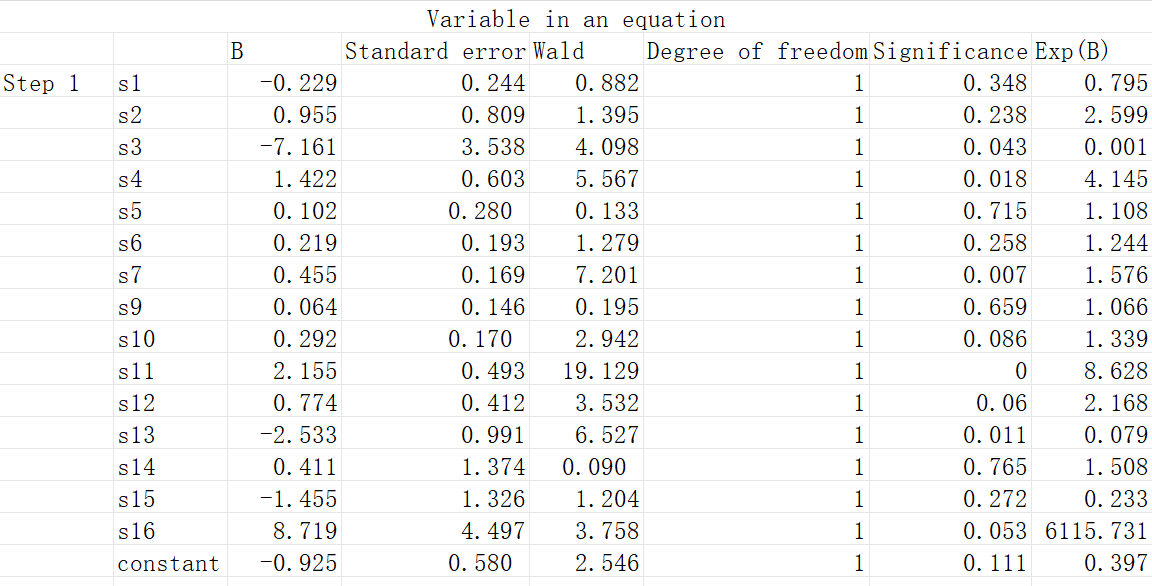
\includegraphics[width=0.7\textwidth]{logistic_eq2.png}
      \caption{Logistic regression results}
\end{figure}
Compared with the results of Question 1, in the existing results, many variables that were originally insignificant became significant, including x3, x4, x11 and x13
\bibliographystyle{alpha}
\bibliography{sample}

\end{document}